\documentclass[final,hyperref={pdfpagelabels=false}]{beamer}
\usepackage{grffile}
\mode<presentation>{\usetheme{I6pd2}}
\usepackage[english]{babel}
\usepackage[latin1]{inputenc}
\usepackage{amsmath,amsthm, amssymb, latexsym}
\usepackage{multirow}
\usepackage{xcolor}
\usepackage{xspace}
\usepackage{textcomp}
%\usepackage{times}\usefonttheme{professionalfonts}  % obsolete
%\usefonttheme[onlymath]{serif}
%\boldmath
\usepackage[orientation=landscape,size=a0,scale=1.4,debug]{beamerposter}
% change list indention level
% \setdefaultleftmargin{3em}{}{}{}{}{}

\newcommand{\GeV}{\textsf{GeV}}

%\usepackage{snapshot} % will write a .dep file with all dependencies, allows for easy bundling

\usepackage{array,booktabs,tabularx}
\newcolumntype{Z}{>{\centering\arraybackslash}X} % centered tabularx columns
\newcommand{\pphantom}{\textcolor{ta3aluminium}} % phantom introduces a vertical space in p formatted table columns??!!

\setbeamertemplate{headline}{  
  \leavevmode

  \begin{beamercolorbox}[wd=\paperwidth]{headline}
    \begin{columns}[T]
      \begin{column}{.02\paperwidth}
      \end{column}
      \begin{column}{.1\paperwidth}
        \vskip4ex
        \begin{center}
          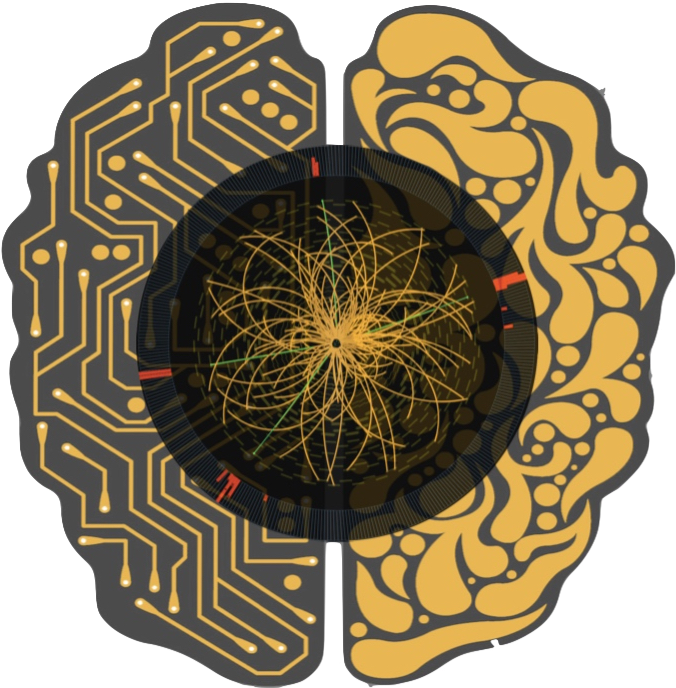
\includegraphics[width=1\linewidth]{figures/fml2.png}
        \end{center}
        \vskip4ex
      \end{column}
      \begin{column}{.715\paperwidth}
        \vskip8ex
        \raggedleft
        \usebeamercolor{title in headline}{\color{fg}\textbf{\huge{\inserttitle}}\\[1ex]}
        \usebeamercolor{author in headline}{\color{fg}\large{\insertauthor}\\[1ex]}
        \usebeamercolor{institute in headline}{\color{fg}\large{\insertinstitute}\\[1ex]}     
      \end{column}
      \begin{column}{.1\paperwidth}
        \vskip4ex
        \begin{center}
          
\includegraphics[width=\linewidth]{figures/iris-hep.png}
        \end{center}
        \vskip4ex
      \end{column}
      \begin{column}{.02\paperwidth}
      \end{column}
    \end{columns}
    \vskip2ex
  \end{beamercolorbox}

  \begin{beamercolorbox}[wd=\paperwidth]{lower separation line head}
    \rule{0pt}{3pt}
  \end{beamercolorbox}
}

\setbeamertemplate{footline}{
  \begin{beamercolorbox}[wd=\paperwidth]{upper separation line foot}
    \rule{0pt}{3pt}
  \end{beamercolorbox}
  
  \leavevmode%
  \begin{beamercolorbox}[ht=4ex,leftskip=1em,rightskip=1em]{author in
      head/foot}%
    \href{https://fastmachinelearning.org}{fastmachinelearning.org}
    \hfill
    \href{https://iris-hep.org}{iris-hep.org}
    \hfill
    \href{https://ml4physicalsciences.github.io/2020}{\textsf{Machine
        Learning and the Physical Sciences, NeurIPS 2020, Vancouver, BC, Canada}}
    \vskip1ex
  \end{beamercolorbox}
  \vskip0pt%
  \begin{beamercolorbox}[wd=\paperwidth]{lower separation line foot}
    \rule{0pt}{3pt}
  \end{beamercolorbox}
}
\setbeamercolor{separation line}{bg=taorange}
\setbeamercolor{title in headline}{fg=taaluminium}
\setbeamercolor{author in headline}{fg=taorange}
\setbeamercolor{author in head/foot}{fg=taorange, bg=black}
\setbeamercolor*{normal text}{fg=tachameleon, bg=white}
\setbeamercolor*{block body}{fg=black,bg=white}
\setbeamercolor*{block title}{fg=taorange,bg=black}
\setbeamerfont{block title}{size=\large,series=\bf}
\setbeamercolor{structure}{fg=ta3skyblue}

\listfiles

%%%%%%%%%%%%%%%%%%%%%%%%%%%%%%%%%%%%%%%%%%%%%%%%%%%%%%%%%%%%%%%%%%%%%%%%%%%%%%%%%%%%%%
%\graphicspath{{figures/}}

\title{Accelerated Charged Particle Tracking with Graph Neural Networks on FPGAs}
\author{
 Aneesh Heintz{\color{lightgray}\inst{1}},
 \textbf{Vesal Razavimaleki}{\color{lightgray}\inst{2}}, \href{https://jduarte.physics.ucsd.edu}{Javier Duarte}{\color{lightgray}\inst{2}}, Gage DeZoort{\color{lightgray}\inst{3}}, Isobel Ojalvo{\color{lightgray}\inst{3}}, Savannah Thais{\color{lightgray}\inst{3}}, Markus Atkinson{\color{lightgray}\inst{4}}, Mark Neubauer{\color{lightgray}\inst{4}}, Lindsey Gray{\color{lightgray}\inst{5}}, Sergo Jindariani{\color{lightgray}\inst{5}}, Nhan Tran{\color{lightgray}\inst{5}}, Phil Harris{\color{lightgray}\inst{6}}, Dylan Rankin{\color{lightgray}\inst{6}}, Thea Aarrestad{\color{lightgray}\inst{7}}, Vladimir Loncar{\color{lightgray}\inst{7}}, Maurizio Pierini{\color{lightgray}\inst{7}}, Sioni Summers{\color{lightgray}\inst{7}}, Jennifer Ngadiuba{\color{lightgray}\inst{8}}, Mia Liu{\color{lightgray}\inst{9}}, Edward Kreinar{\color{lightgray}\inst{10}}, Zhenbin Wu{\color{lightgray}\inst{11}}}
\institute{\color{lightgray}\inst{1} Cornell \inst{2} UC San Diego \inst{3} Princeton \inst{4} UIUC \inst{5} Fermilab \inst{6} MIT \inst{7} CERN \inst{8} Caltech \inst{9} Purdue \inst{10} Hawkeye360 \inst{11} UIC}
\date[December 11, 2020]{December 11, 2020}

%%%%%%%%%%%%%%%%%%%%%%%%%%%%%%%%%%%%%%%%%%%%%%%%%%%%%%%%%%%%%%%%%%%%%%%%%%%%%%%%%%%%%%
\newlength{\columnheight}
\setlength{\columnheight}{105cm}

\newcommand{\hlsfml}{{\texttt{hls4ml}}\xspace}
\newcommand{\pt}{\ensuremath{p_{\mathrm{T}}}\xspace}
\newcommand{\ptmin}{\ensuremath{p_{\mathrm{T_{min}}}}\xspace}

%%%%%%%%%%%%%%%%%%%%%%%%%%%%%%%%%%%%%%%%%%%%%%%%%%%%%%%%%%%%%%%%%%%%%%%%%%%%%%%%%%%%%%
\begin{document}
\begin{frame}
  \begin{columns}
    % ---------------------------------------------------------%
    % Set up a column 
    \begin{column}{.33\textwidth}
      \begin{beamercolorbox}[center,wd=\textwidth]{postercolumn}
        \begin{minipage}[T]{.95\textwidth}  % tweaks the width, makes a new \textwidth
          \parbox[t][\columnheight]{\textwidth}{ % must be some better way to set the the height, width and textwidth simultaneously
            % Since all columns are the same length, it is all nice and tidy.  You have to get the height empirically
            % ---------------------------------------------------------%
            % fill each column with content
            
            \begin{block}{Introduction}
              \vspace{-1.65cm}
              \begin{columns}
              \begin{column}{.49\textwidth}
                \begin{itemize}
                  \item Tracking approached as a graph ``edge classification'' problem
                  \item Data represented as graphs
                  \begin{itemize}
                    \item Nodes$\,\to\,$Hits
                    \item Edges$\,\to\,$Doublet connections
                  \end{itemize}
                  \item Interest in GNN inference in FPGA-based trigger and co-processors to improve offline computational performance
                  \item FPGA implementations of GNN segment classifiers explored using \hlsfml and OpenCL
                  \item \href{https://github.com/fastmachinelearning/hls4ml}{\hlsfml}: compiler for physicists and ML experts to convert ML algorithms into FPGA firmware
                  \item OpenCL: framework for writing programs that execute across heterogenous platforms (CPUs, GPUs, FPGAs, etc.)
                \end{itemize}
              \end{column}
              \begin{column}{.49\textwidth}
                \begin{center}
                  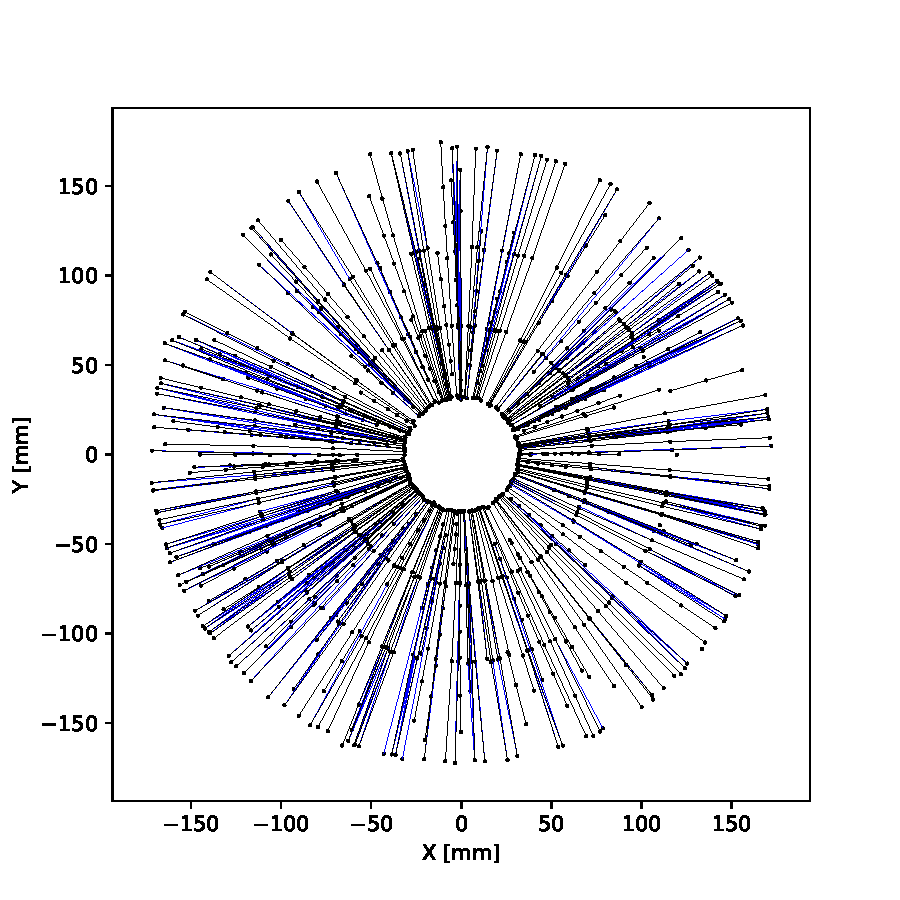
\includegraphics[width=0.85\linewidth]{figures/event000001000_section0_xy.pdf}
                  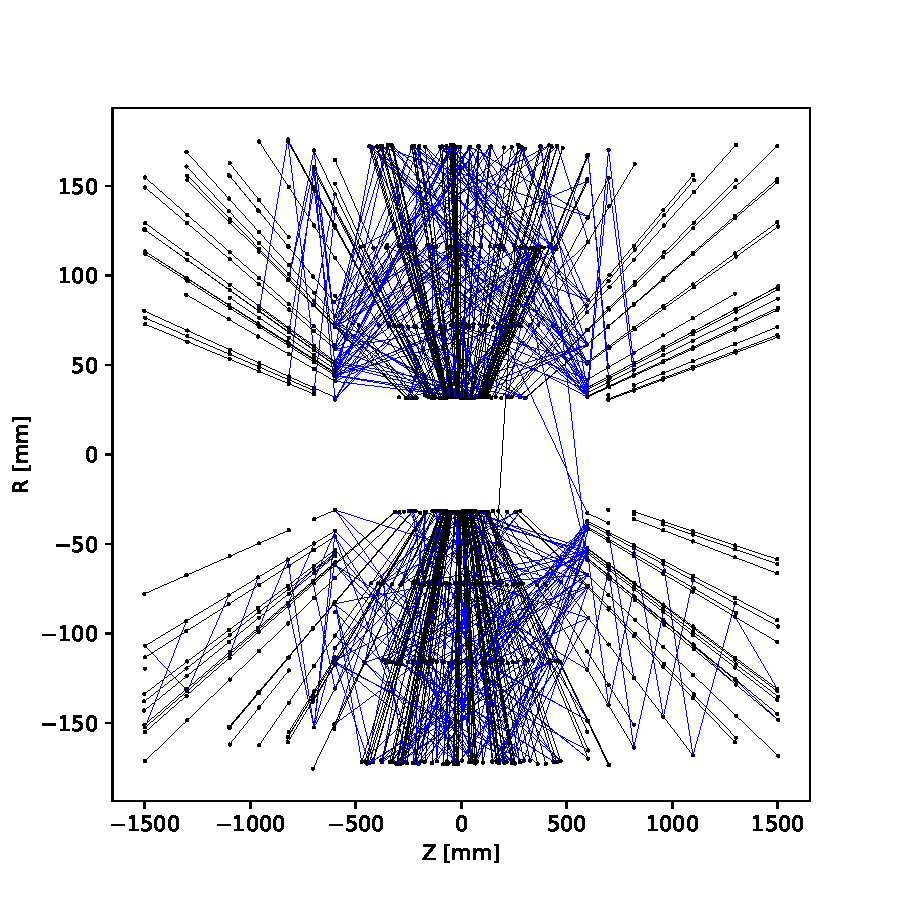
\includegraphics[width=0.85\linewidth]{figures/event000001000_section0_rz.pdf}
                \end{center}
              \end{column}
              \end{columns}
            \end{block}\vspace{-2cm}
            
            \begin{block}{Model Architectures}
              \begin{itemize}
              \item \hlsfml Implementation
              \begin{itemize}
                  \item Architecture: \href{https://arxiv.org/abs/2003.11603}{Exa.TrkX NeurIPS 2019 Segment Classifier}
                  \item Encoder (edges/nodes): 4/3$\,\to\,$(8, 8)
                  \item Interaction Network (edge and node blocks): 8$\,\to\,$(8, 8)
                  \item Decoder (edges): 8$\,\to\,$(8, 8, 8, 1)
              \end{itemize}
              \end{itemize}
              \begin{center}
                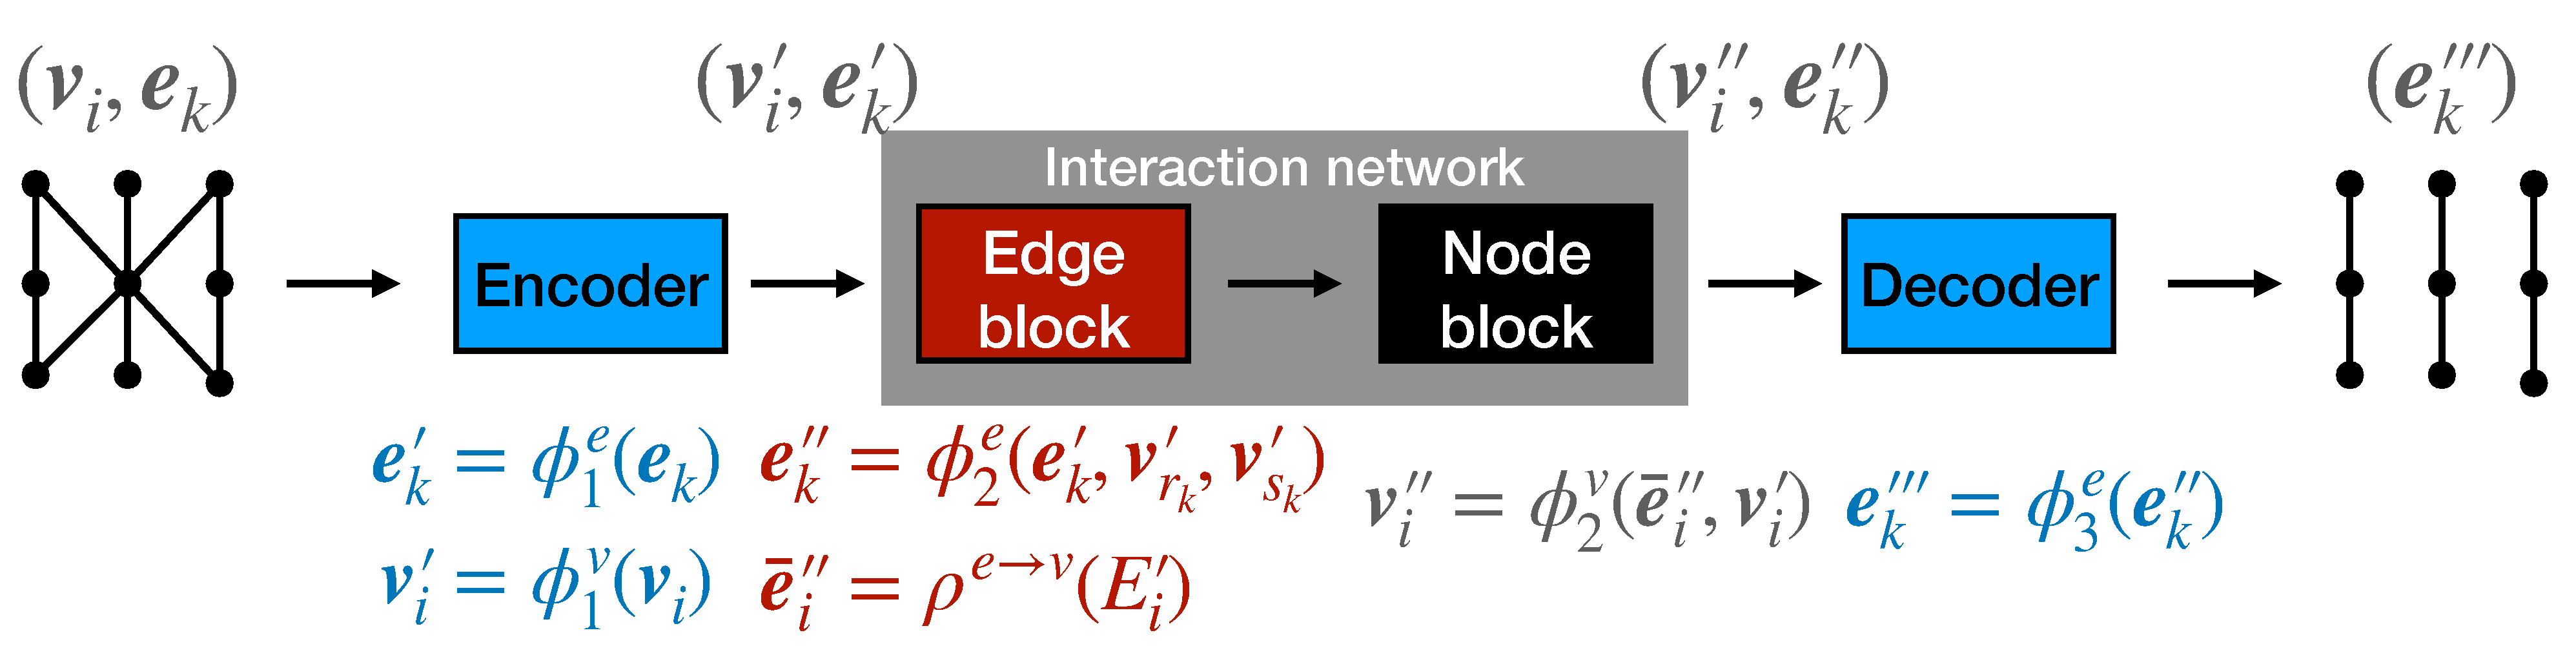
\includegraphics[height=0.2\linewidth]{figures/hls4ml_GNN_resize.pdf}
              \end{center}
              \begin{itemize}
              \item OpenCL Implementation
              \begin{itemize}
                  \item Architecture: Interaction Network
                  \item Edge block: 7$\,\to\,$(250, 250, 250, 1), node block: 4$\,\to\,$(200, 200, 3)
              \end{itemize}
              \end{itemize}
              \begin{center}  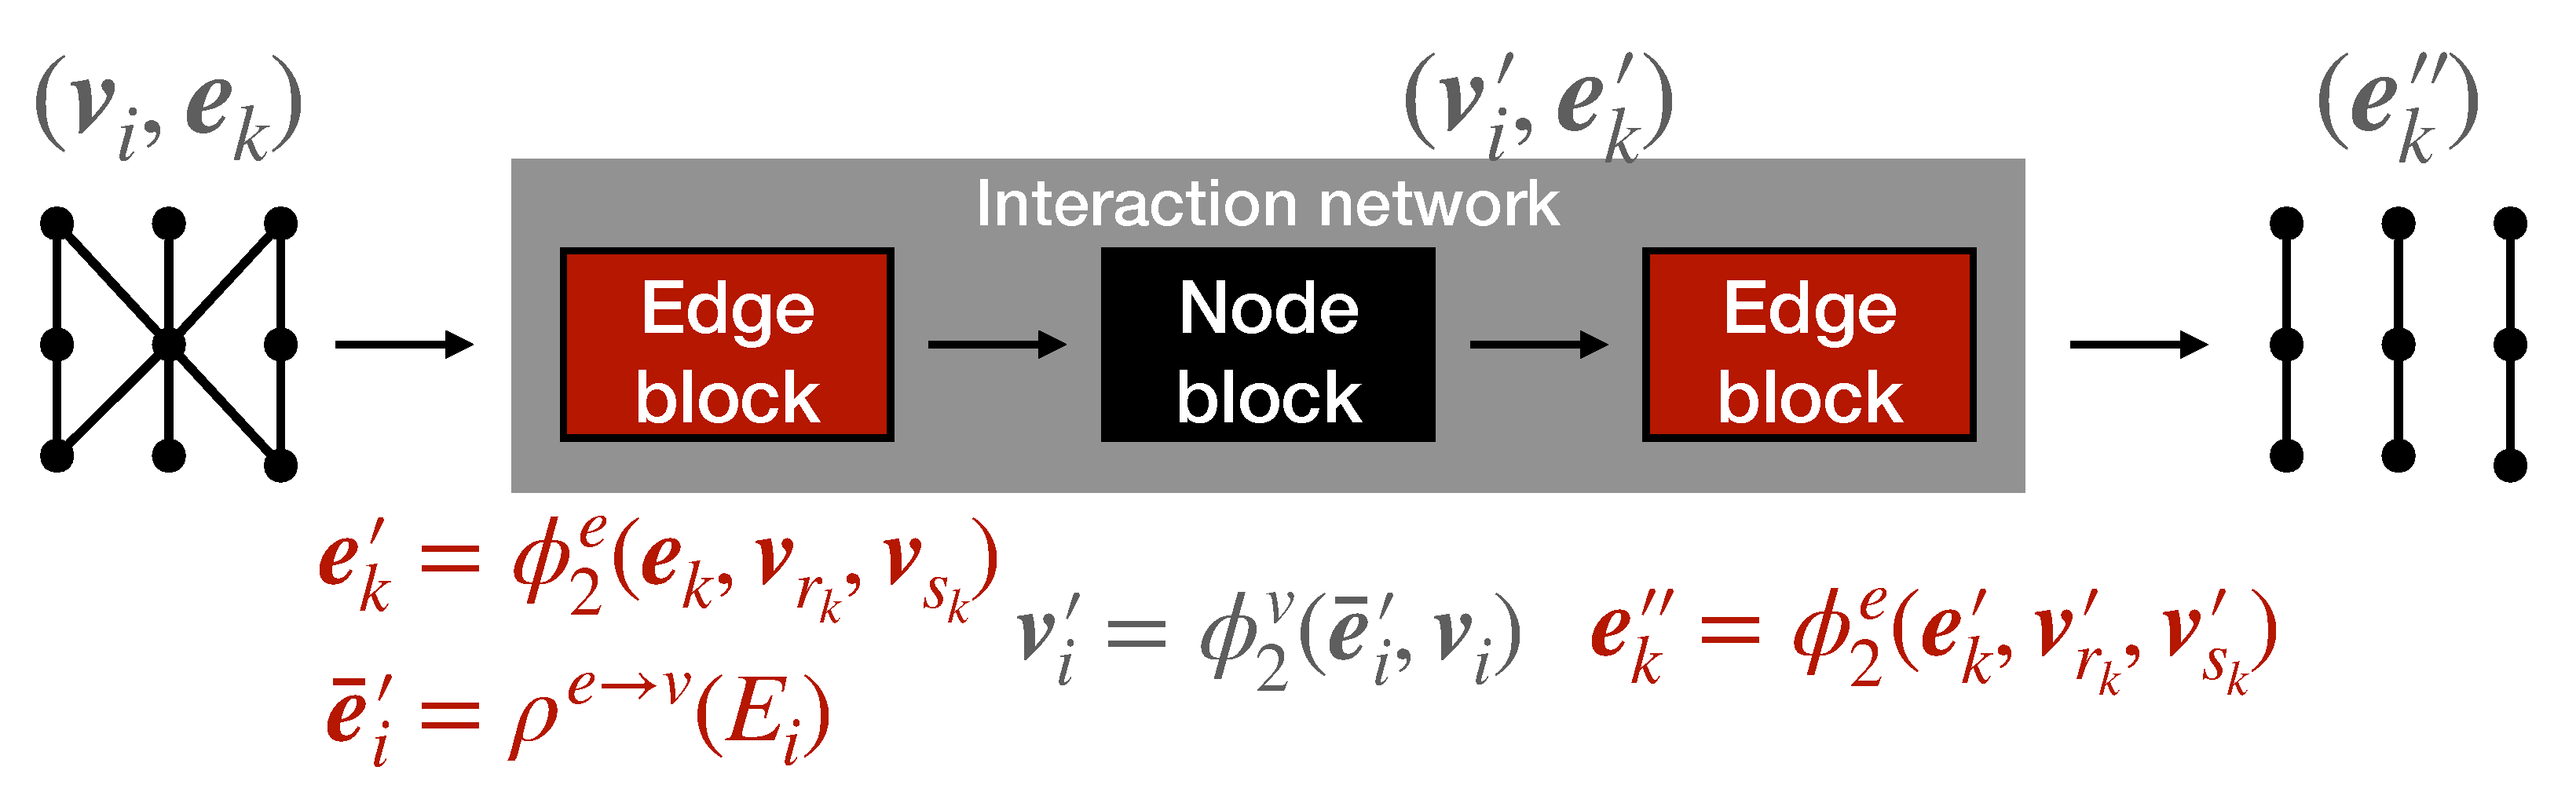
\includegraphics[height=0.2\linewidth]{figures/OpenCL_GNN_resize.pdf}
              \end{center}
            \end{block}
                }
              \end{minipage}
            \end{beamercolorbox}
          \end{column}
    % ---------------------------------------------------------%
    % end the column

    % ---------------------------------------------------------%
    % Set up a column 
    \begin{column}{.33\textwidth}
      \begin{beamercolorbox}[center,wd=\textwidth]{postercolumn}
        \begin{minipage}[T]{.95\textwidth} 
          \parbox[t][\columnheight]{\textwidth}{
            
            \begin{block}{\hlsfml Latency and Resources}
              \begin{itemize}
                \item Efficiency improvements for design targeting Xilinx KU115 FPGA:
                \begin{itemize}
                    \item Pipelining with reuse factor at edge/node block-level
                    \item Input streaming: implement incoming data as FIFO to recycle resources
                    \item Loop unrolling, zero-padding up to max. graph size
                \end{itemize}
                \item For 1/64 of TrackML detector, \ptmin = 2~GeV (28 nodes, 37 edges at 95th percentile)
                \item Achieves latency of 650~ns to 1~$\mu$s
                \item Scan vs. bit precision show lower bit width results in smaller area, faster execution
                \begin{center}
                    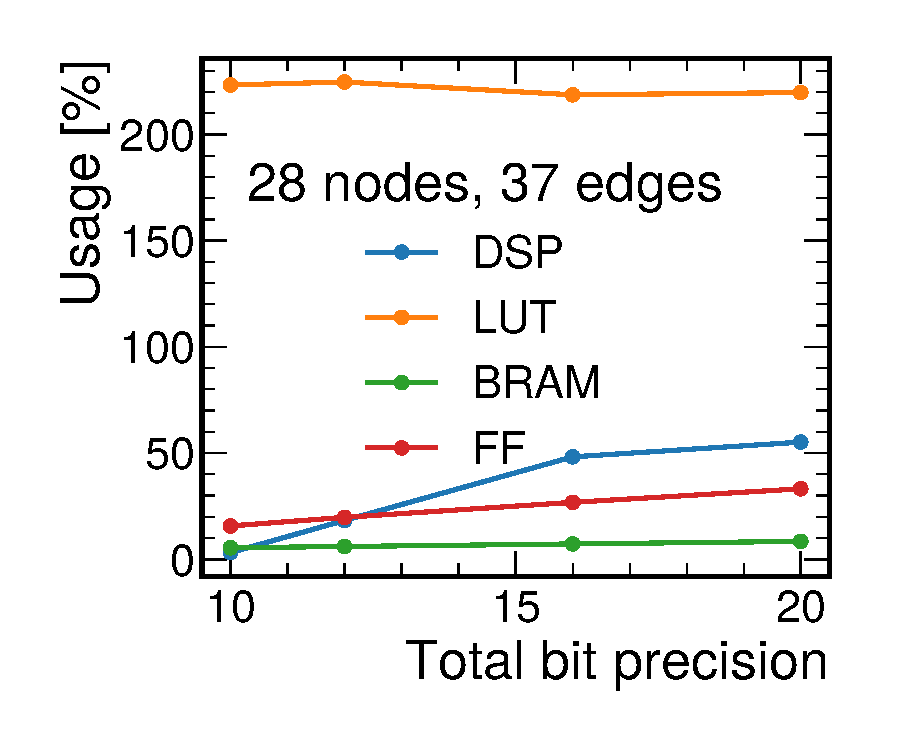
\includegraphics[width=0.49\linewidth]{figures/Resources_vs_BP.pdf}
                    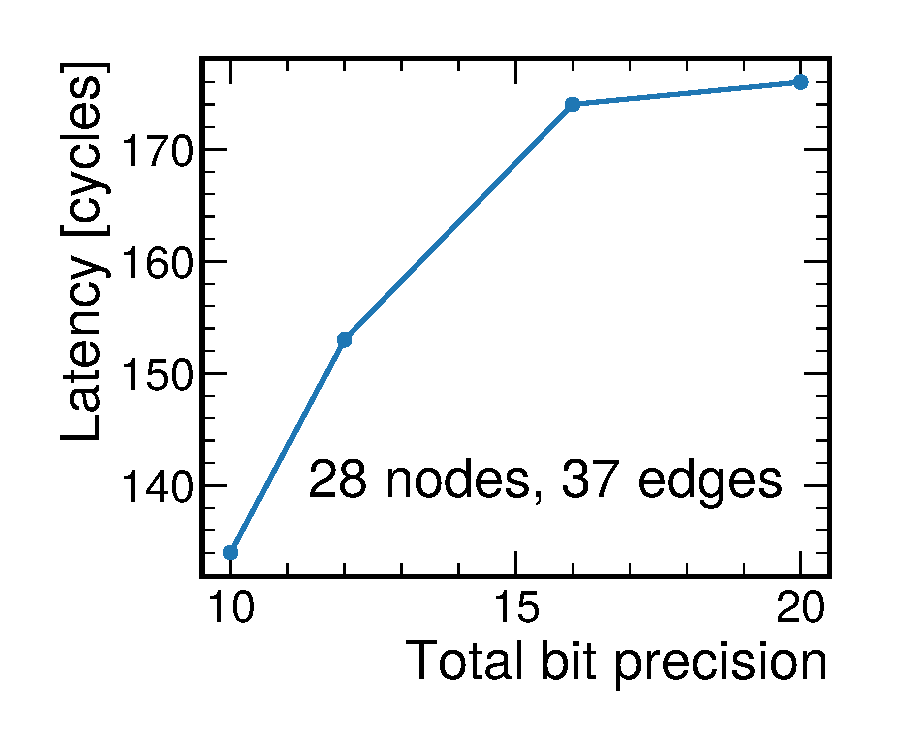
\includegraphics[width=0.49\linewidth]{figures/Latency_vs_BP.pdf}
                \end{center}
                \item Scan vs. reuse factor show trade-off between resource usage and latency
                \begin{center}
                    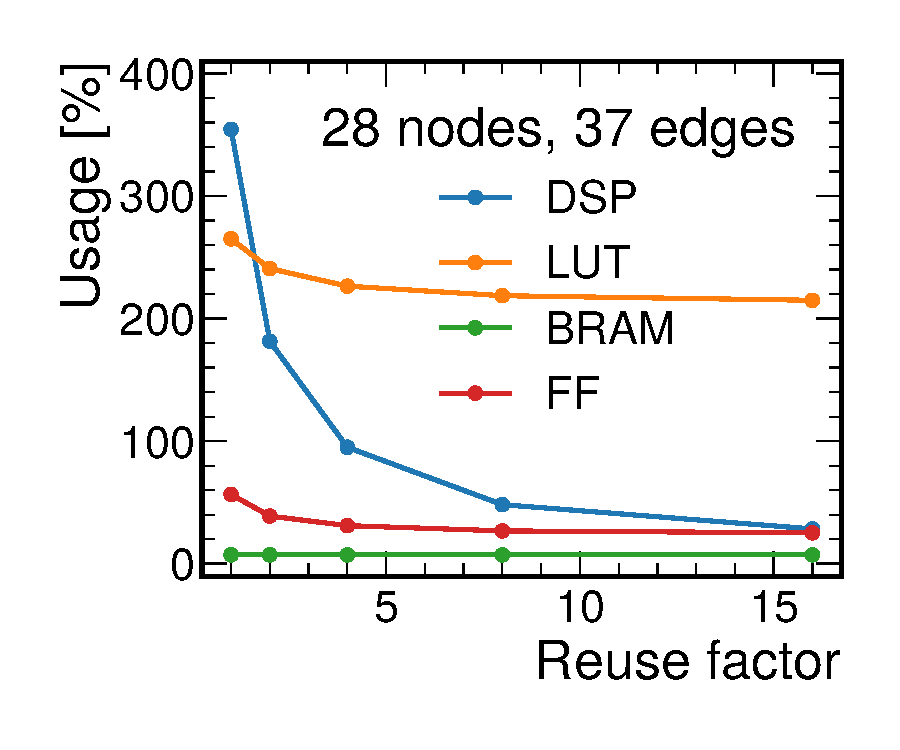
\includegraphics[width=0.49\linewidth]{figures/Resources_vs_RF.pdf}
                    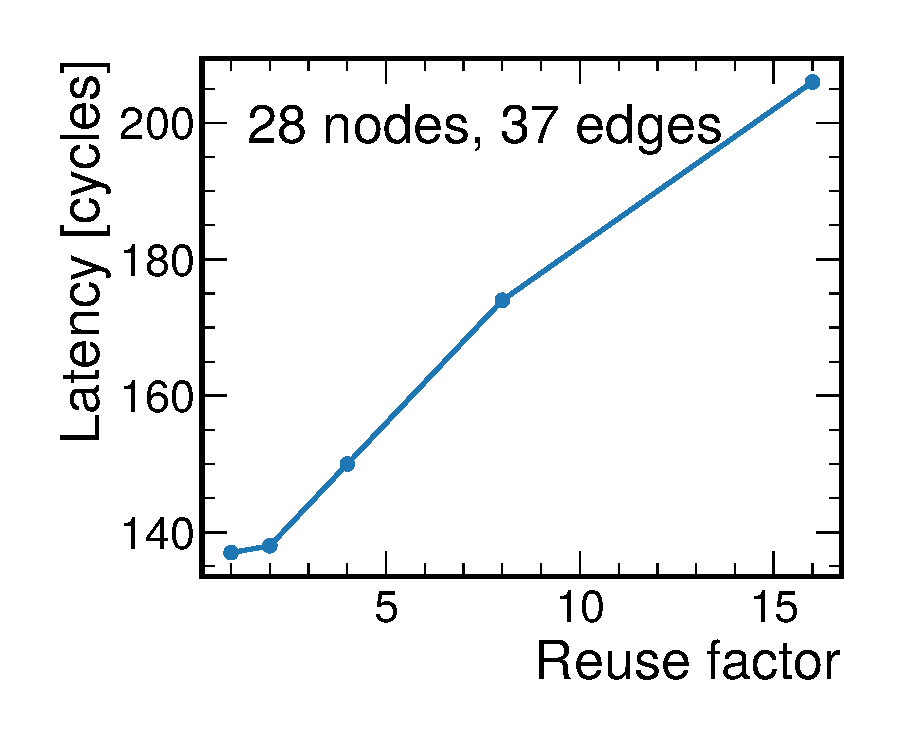
\includegraphics[width=0.49\linewidth]{figures/Latency_vs_RF.pdf}
                \end{center}
              \end{itemize}
            \end{block}\vspace{-2cm}
            
            \begin{block}{\hlsfml Performance}
              \vspace{-1.2cm}
              \begin{columns}
                \begin{column}{.49\textwidth}
                  \begin{itemize}
                   \item GNN correctly classifies track segments with AUC $\sim$ 0.983
                  \item AUC scan vs. fixed-point bit precision \texttt{<total,integer>} shows good performance for \texttt{<12,6>}
                      \item For 1/16 of a TrackML detector, \ptmin = 2~GeV (112 nodes, 148 edges at 95th percentile)
                  \end{itemize}
                \end{column}
                \begin{column}{.49\textwidth}
                  \begin{center}
                      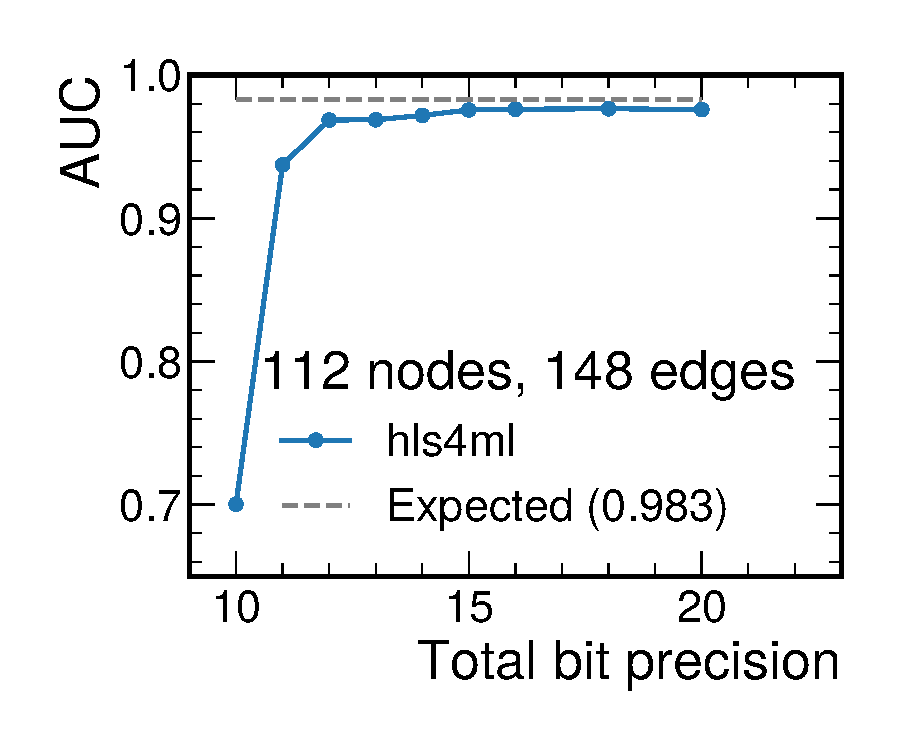
\includegraphics[width=\linewidth]{figures/AUC_vs_BP.pdf}
                  \end{center}
                \end{column}
              \end{columns}
              \vspace{-1.3cm}
            \end{block}
                }
              \end{minipage}
            \end{beamercolorbox}
          \end{column}
    % ---------------------------------------------------------%
    % end the column

    % ---------------------------------------------------------%
    % Set up a column 
    \begin{column}{.33\textwidth}
      \begin{beamercolorbox}[center,wd=\textwidth]{postercolumn}
        \begin{minipage}[T]{.95\textwidth} 
          \parbox[t][\columnheight]{\textwidth}{
            
            \begin{block}{OpenCL Latency and Resources}
            \begin{columns}
             \begin{column}{.49\textwidth}
              \begin{itemize}
                \item Efficiency improvements for design targeting Arria 10 GX 1150 FPGA:
                \begin{itemize}
                    \item 2D local memory tiling/register blocking: reduce redundancy/latency of reading off-chip memory
                    \item Double buffering: allow host to process/transfer data while kernel executes
                    \item Loop unrolling
                \end{itemize}
                \item Scales up more easily to larger graph sizes (smaller \ptmin)
                \item Achieves latency of 10~ms to 1~s including CPU-FPGA I/O  
              \end{itemize}
              \end{column}
             \begin{column}{.49\textwidth}
                \begin{center}         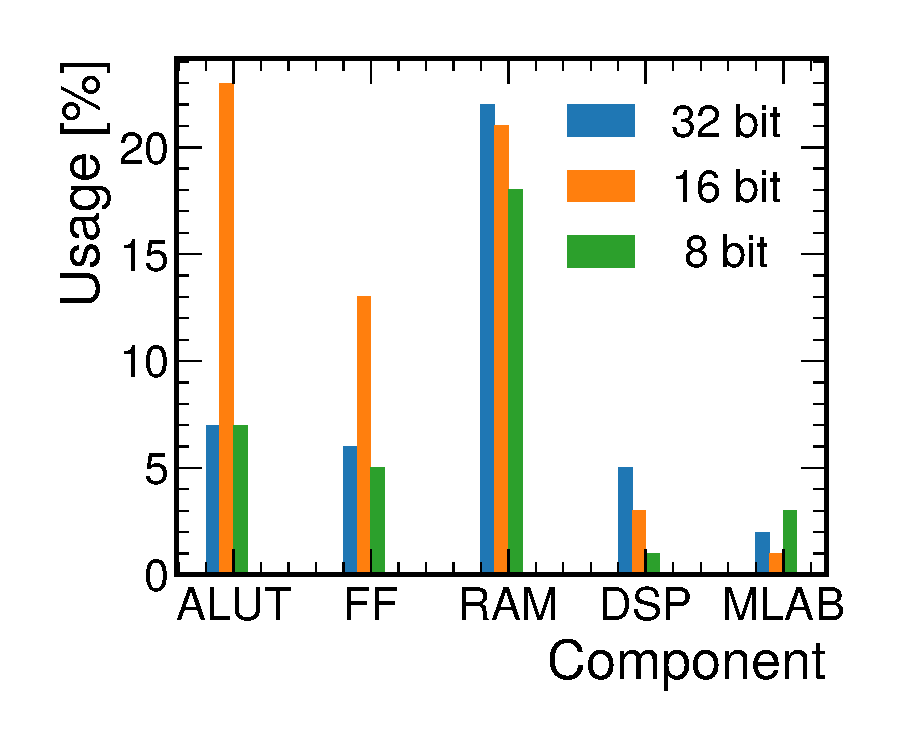
\includegraphics[width=\linewidth]{figures/resource_bit_precision_ocl.pdf}
                \end{center}
               \end{column}
              \end{columns}
                \begin{center}    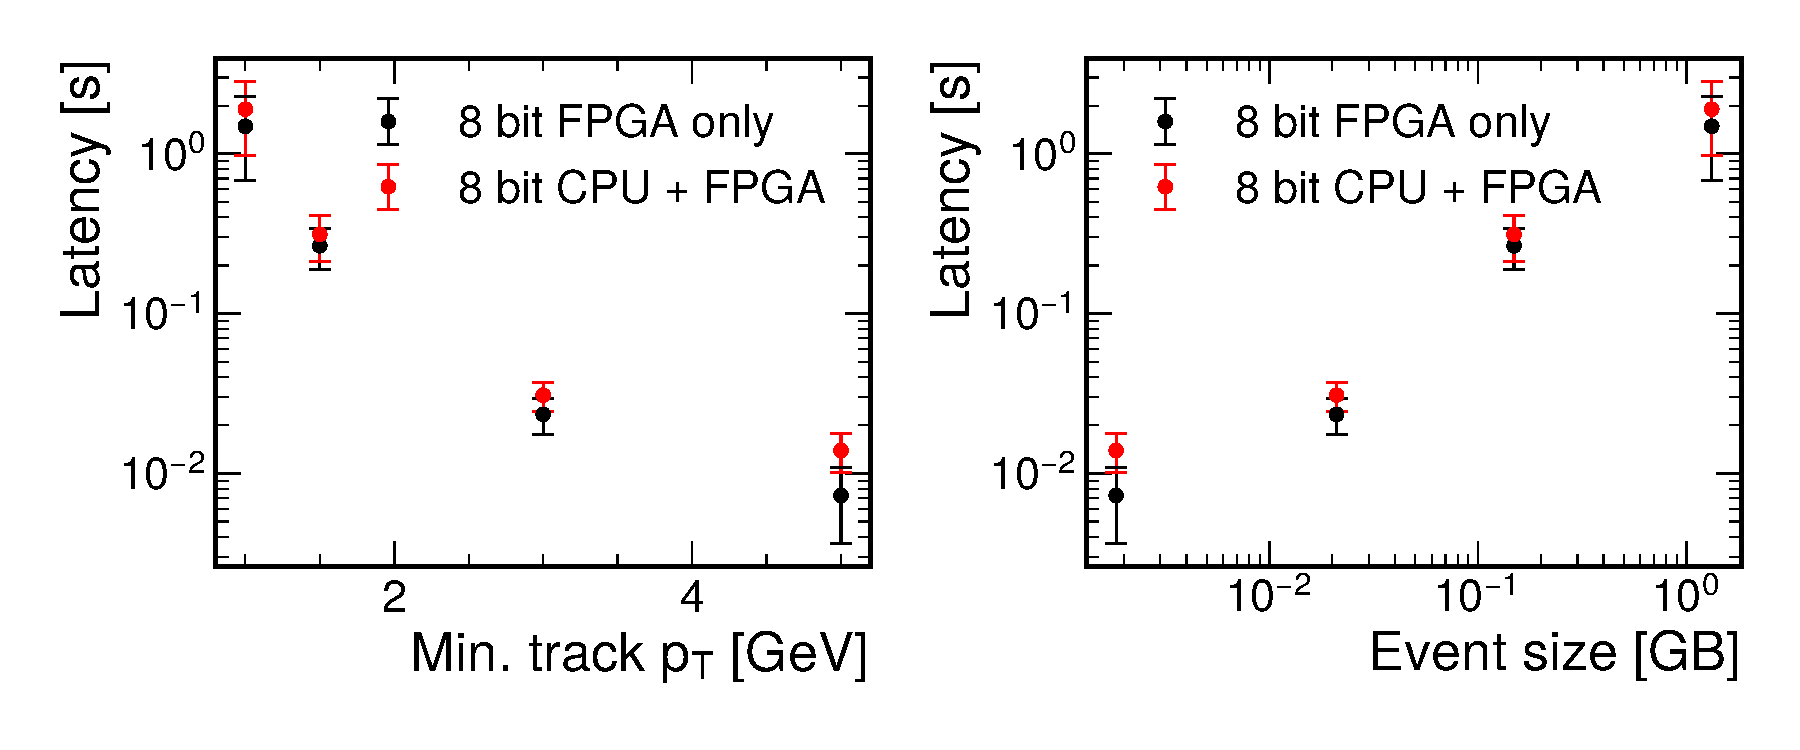
\includegraphics[width=\linewidth]{figures/scalability_study_v2.pdf}
                \end{center}
            \end{block}\vspace{-2cm}
            \begin{block}{Summary}
              \begin{itemize}
                \item Two complementary implementations of GNNs on FPGAs
                \item Current performance promising for trigger-level applications (\hlsfml) and co-processing applications (OpenCL and \hlsfml)
                \item OpenCL implementation scales more easily to larger \\graphs while \hlsfml implementation has\\ latency/throughput advantage
                \item Future Work
                \begin{itemize}
                    \item Further detailed comparisons between the implementations based\\ on the same model
                    \item Comparison with GPU co-processors
                    \item Additional optimizations such as quantization-aware training
                \end{itemize}
              \end{itemize}       \begin{flushright}
              \vspace{-20ex} \href{https://arxiv.org/abs/2012.01563}{
\includegraphics[width=0.18\textwidth]{figures/gnn_fpga_qr_code.png}}\\
                             \includegraphics[width=0.05\linewidth]{figures/ScullyComputer.jpg}
                          \end{flushright}
            \end{block}                  
                }
              \end{minipage}
            \end{beamercolorbox}
          \end{column}
    % ---------------------------------------------------------%
    % end the column

    % ---------------------------------------------------------%
    % end the column
  \end{columns}
  \vskip1ex

\end{frame}
\end{document}


%%%%%%%%%%%%%%%%%%%%%%%%%%%%%%%%%%%%%%%%%%%%%%%%%%%%%%%%%%%%%%%%%%%%%%%%%%%%%%%%%%%%%%%%%%%%%%%%%%%%
%%% Local Variables: 
%%% mode: latex
%%% TeX-PDF-mode: t
%%% End: